\documentclass[12pt,twoside]{report}
\usepackage{tikz}
\usetikzlibrary{positioning, fit, arrows.meta}

%%%%%%%%%%%%%%%%%%%%%%%%%%%%%%%%%%%%%%%%%%%%%%%%%%%%%%%%%%%%%%%%%%%%%%%%%%%%%

% Definitions for the title page
% Edit these to provide the correct information
% e.g. \newcommand{\reportauthor}{Timothy Kimber}

\newcommand{\reporttitle}{Chameleon Text: Exploring ways to increase variety in artificial data}
\newcommand{\reportauthor}{Thien P. Nguyen}
\newcommand{\supervisor}{Lucia Specia}
\newcommand{\degreetype}{Computing (Artificial Intelligence)}

%%%%%%%%%%%%%%%%%%%%%%%%%%%%%%%%%%%%%%%%%%%%%%%%%%%%%%%%%%%%%%%%%%%%%%%%%%%%%

% load some definitions and default packages
%%%%%%%%%%%%%%%%%%%%%%%%%%%%%%%%%%%%%%%%%
% University Assignment Title Page 
% LaTeX Template
% Version 1.0 (27/12/12)
%
% This template has been downloaded from:
% http://www.LaTeXTemplates.com
%
% Original author:
% WikiBooks (http://en.wikibooks.org/wiki/LaTeX/Title_Creation)
%
% License:
% CC BY-NC-SA 3.0 (http://creativecommons.org/licenses/by-nc-sa/3.0/)
% 
%
%%%%%%%%%%%%%%%%%%%%%%%%%%%%%%%%%%%%%%%%%
%----------------------------------------------------------------------------------------
%	PACKAGES AND OTHER DOCUMENT CONFIGURATIONS
%----------------------------------------------------------------------------------------
\usepackage[a4paper,hmargin=2.3cm,vmargin=2.0cm,includeheadfoot]{geometry}
\usepackage{textpos}
\usepackage{natbib} % for bibliography
\usepackage{tabularx,longtable,multirow,subfigure,caption}%hangcaption
\usepackage{fncylab} %formatting of labels
\usepackage{fancyhdr} % page layout
\usepackage{url} % URLs
\usepackage[english]{babel}
\usepackage{amsmath}
\usepackage{graphicx}
\usepackage{dsfont}
\usepackage{epstopdf} % automatically replace .eps with .pdf in graphics
\usepackage{backref} % needed for citations
\usepackage{array}
\usepackage{latexsym}
\usepackage[pdftex,pagebackref,hypertexnames=false,colorlinks]{hyperref} % provide links in pdf

\hypersetup{pdftitle={},
  pdfsubject={}, 
  pdfauthor={},
  pdfkeywords={}, 
  pdfstartview=FitH,
  pdfpagemode={UseOutlines},% None, FullScreen, UseOutlines
  bookmarksnumbered=true, bookmarksopen=true, colorlinks,
    citecolor=black,%
    filecolor=black,%
    linkcolor=black,%
    urlcolor=black}

\usepackage[all]{hypcap}


%\usepackage{color}
%\usepackage[tight,ugly]{units}
%\usepackage{float}
%\usepackage{tcolorbox}
%\usepackage[colorinlistoftodos]{todonotes}
% \usepackage{ntheorem}
% \theoremstyle{break}
% \newtheorem{lemma}{Lemma}
% \newtheorem{theorem}{Theorem}
% \newtheorem{remark}{Remark}
% \newtheorem{definition}{Definition}
% \newtheorem{proof}{Proof}


%%% Default fonts
\renewcommand*{\rmdefault}{bch}
\renewcommand*{\ttdefault}{cmtt}



%%% Default settings (page layout)
\setlength{\parindent}{0em}  % indentation of paragraph

\setlength{\headheight}{14.5pt}
\pagestyle{fancy}
\renewcommand{\chaptermark}[1]{\markboth{\chaptername\ \thechapter.\ #1}{}} 

\fancyfoot[ER,OL]{\sffamily\textbf{\thepage}}%Page no. in the left on odd pages and on right on even pages
\fancyfoot[OC,EC]{\sffamily }
\renewcommand{\headrulewidth}{0.1pt}
\renewcommand{\footrulewidth}{0.1pt}
\captionsetup{margin=10pt,font=small,labelfont=bf}


%--- chapter heading

\def\@makechapterhead#1{%
  \vspace*{10\p@}%
  {\parindent \z@ \raggedright \sffamily
    \interlinepenalty\@M
    \Huge\bfseries \thechapter \space\space #1\par\nobreak
    \vskip 30\p@
  }}

%---chapter heading for \chapter*  
\def\@makeschapterhead#1{%
  \vspace*{10\p@}%
  {\parindent \z@ \raggedright
    \sffamily
    \interlinepenalty\@M
    \Huge \bfseries  #1\par\nobreak
    \vskip 30\p@
  }}

\allowdisplaybreaks

% load some macros
% Here, you can define your own macros. Some examples are given below.

\newcommand{\R}[0]{\mathds{R}} % real numbers
\newcommand{\Z}[0]{\mathds{Z}} % integers
\newcommand{\N}[0]{\mathds{N}} % natural numbers
\newcommand{\C}[0]{\mathds{C}} % complex numbers
\renewcommand{\vec}[1]{{\boldsymbol{{#1}}}} % vector
\newcommand{\mat}[1]{{\boldsymbol{{#1}}}} % matrix


\date{May 2019}

\begin{document}

% load title page
% Last modification: 2015-08-17 (Marc Deisenroth)
\begin{titlepage}

\newcommand{\HRule}{\rule{\linewidth}{0.5mm}} % Defines a new command for the horizontal lines, change thickness here


%----------------------------------------------------------------------------------------
%	LOGO SECTION
%----------------------------------------------------------------------------------------


\includegraphics[width = 4cm]{./figures/imperial}\\[0.5cm] 

\center % Center remainder of the page

%----------------------------------------------------------------------------------------
%	HEADING SECTIONS
%----------------------------------------------------------------------------------------

\textsc{\Large Imperial College London}\\[0.5cm] 
\textsc{\large Department of Computing}\\[0.5cm] 

%----------------------------------------------------------------------------------------
%	TITLE SECTION
%----------------------------------------------------------------------------------------

\HRule \\[0.4cm]
{ \huge \bfseries \reporttitle}\\ % Title of your document
\HRule \\[1.5cm]
 
%----------------------------------------------------------------------------------------
%	AUTHOR SECTION
%----------------------------------------------------------------------------------------

\begin{minipage}{0.4\textwidth}
\begin{flushleft} \large
\emph{Author:}\\
\reportauthor % Your name
\end{flushleft}
\end{minipage}
~
\begin{minipage}{0.4\textwidth}
\begin{flushright} \large
\emph{Supervisor:} \\
\supervisor % Supervisor's Name
\end{flushright}
\end{minipage}\\[4cm]


%----------------------------------------------------------------------------------------
%	FOOTER & DATE SECTION
%----------------------------------------------------------------------------------------
\vfill % Fill the rest of the page with whitespace
Submitted in partial fulfillment of the requirements for the MSc degree in
\degreetype~of Imperial College London\\[0.5cm]

\makeatletter
\@date 
\makeatother


\end{titlepage}



% page numbering etc.
\pagenumbering{roman}
\clearpage{\pagestyle{empty}\cleardoublepage}
\setcounter{page}{1}
\pagestyle{fancy}

%%%%%%%%%%%%%%%%%%%%%%%%%%%%%%%%%%%%
% \begin{abstract}
% Your abstract.
% \end{abstract}

% \cleardoublepage
%%%%%%%%%%%%%%%%%%%%%%%%%%%%%%%%%%%%
% \section*{Acknowledgments}
% Comment this out if not needed.

% \clearpage{\pagestyle{empty}\cleardoublepage}

%%%%%%%%%%%%%%%%%%%%%%%%%%%%%%%%%%%%
%--- table of contents
% \fancyhead[RE,LO]{\sffamily {Table of Contents}}
% \tableofcontents 


% % \clearpage{\pagestyle{empty}\cleardoublepage}
\pagenumbering{arabic}
\setcounter{page}{1}
\fancyhead[LE,RO]{\slshape \rightmark}
\fancyhead[LO,RE]{\slshape \leftmark}

%%%%%%%%%%%%%%%%%%%%%%%%%%%%%%%%%%%%
% \chapter{Introduction}

% \begin{figure}[tb]
% \centering
% 
\includegraphics[width = 0.4\hsize]{./figures/imperial}
% \caption{Imperial College Logo. It's nice blue, and the font is quite stylish. But you can choose a different one if you don't like it.}
% \label{fig:logo}
% \end{figure}

% Figure~\ref{fig:logo} is an example of a figure. 

%%%%%%%%%%%%%%%%%%%%%%%%%%%%%%%%%%%%
\chapter{Literature Survey}

\section{Background}

\subsection{Neural Networks}

Neural Networks are non-linear statistical models that generate complex relationships between input and output vectors. Note that the input and output vectors are of a fixed dimension, which becomes a problem for our task at hand.

\subsection{Backpropagation}

\subsection{Autoencoders}

Autoencoders are a specialised form of MLPs where the model attempts to recreate the inputs on the output. Autoencoders typically have a neural network layer in the model where its dimension is smaller than the input space, therefore representing a dimensionality reduction in the data. Autoencoders are composed of two different networks, an encoder $\alpha$ and a decoder $\beta$, such that $\alpha : X \rightarrow F$ and $\beta : F \rightarrow X$. The two networks are trained together in a manner that allows them to preserve the input as much as possible.

Increasing the robustness of Autoencoders typically includes the introduction of noise (that the Autoencoder would attempt to ignore - this particular model is described as a Denoising Autoencoder), and experimentation of 

Autoencoders are popularised through their use in Machine Translation, Word Embeddings, and document clustering.

\subsection{Recurrent Neural Networks}

Recurrent neural networks (CNNs) are a particular class of neural networks such that the outputs are not necessarily restricted and discrete (as opposed to the MLP). CNNs essentially operate over a sequence of vectors, making them popular in contempoary NLP problems. Given a sequence of inputs $(x_1, ..., x_T)$, a standard RNN computes a sequence of outputs $(y_1, ..., y_T)$ by iterating the following equation:

\subsubsection{LSTM}

\begin{figure}
	\centering
	\begin{tikzpicture}[
		prod/.style={circle, draw, inner sep=0pt},
		ct/.style={circle, draw, inner sep=5pt, ultra thick, minimum width=10mm},
		ft/.style={circle, draw, minimum width=8mm, inner sep=1pt},
		filter/.style={circle, draw, minimum width=7mm, inner sep=1pt, path picture={\draw[thick, rounded corners] (path picture bounding box.center)--++(65:2mm)--++(0:1mm);
		\draw[thick, rounded corners] (path picture bounding box.center)--++(245:2mm)--++(180:1mm);}},
		mylabel/.style={font=\scriptsize\sffamily},
		>=LaTeX
		]
	
	\node[ct, label={[mylabel]Cell}] (ct) {$c_t$};
	\node[filter, right=of ct] (int1) {};
	\node[prod, right=of int1] (x1) {$\times$}; 
	\node[right=of x1] (ht) {$h_t$};
	\node[prod, left=of ct] (x2) {$\times$}; 
	\node[filter, left=of x2] (int2) {};
	\node[prod, below=5mm of ct] (x3) {$\times$}; 
	\node[ft, below=5mm of x3, label={[mylabel]right:Forget Gate}] (ft) {$f_t$};
	\node[ft, above=of x2, label={[mylabel]left:Input Gate}] (it) {$i_t$};
	\node[ft, above=of x1, label={[mylabel]left:Output Gate}] (ot) {$o_t$};
	
	\foreach \i/\j in {int2/x2, x2/ct, ct/int1, int1/x1,
				x1/ht, it/x2, ct/it, ct/ot, ot/x1, ft/x3}
		\draw[->] (\i)--(\j);
	
	\draw[->] (ct) to[bend right=45] (ft);
	
	\draw[->] (ct) to[bend right=30] (x3);
	\draw[->] (x3) to[bend right=30] (ct);
	
	\node[fit=(int2) (it) (ot) (ft), draw, inner sep=0pt] (fit) {};
	
	\draw[<-] (fit.west|-int2) coordinate (aux)--++(180:7mm) node[left]{$x_t$};
	\draw[<-] ([yshift=1mm]aux)--++(135:7mm);
	\draw[<-] ([yshift=-1mm]aux)--++(-135:7mm);
	
	\draw[<-] (fit.north-|it) coordinate (aux)--++(90:7mm) node[above]{$x_t$};
	\draw[<-] ([xshift=1mm]aux)--++(45:7mm);
	\draw[<-] ([xshift=-1mm]aux)--++(135:7mm);
	
	\draw[<-] (fit.north-|ot) coordinate (aux)--++(90:7mm) node[above]{$x_t$};
	\draw[<-] ([xshift=1mm]aux)--++(45:7mm);
	\draw[<-] ([xshift=-1mm]aux)--++(135:7mm);
	
	\draw[<-] (fit.south-|ft) coordinate (aux)--++(-90:7mm) node[below]{$x_t$};
	\draw[<-] ([xshift=1mm]aux)--++(-45:7mm);
	\draw[<-] ([xshift=-1mm]aux)--++(-135:7mm);
	\end{tikzpicture}
	\caption{A diagram of the LSTM model.}
\end{figure}

LSTM (Long Short Term Memory) is a type of Recurrent Neural Network that attempts to retain information based on the previous inputs through the introduction of gated architectures.

\subsubsection{Gated Recurrent Networks}

GRUs are used to solve the common issue with LSTMs where the training time was relatively slow due to the number of derivatives necessary to compute. Within the GRU architecture, a feature to retain the previous weights remain, but there exists an direct path to the input data from the output, allowing a reduction in training time.

\section{Related Work}

\subsection{Seq2Seq}

Seq2Seq, introduced by \cite{sutskever_sequence_2014} is a modern interpretation of the encoder model, by providing an attention mechanism. The attention mechanism looks at all of the inputs from the hidden states of the encoders so far. 

Traditionally, Seq2seq would be the most common method of tackling this particular problem, but it also presents problems that make it suboptimal. Firstly, it's discrete nature suggests that it is prone to noise in a similar fashion to how linear regression is not necessarily optimal as opposed to 

\subsection{Transformers}


\subsection{Variational Autoencoders}

Variational Autoencoders (VAEs) introduce a constraint on the encoding network that forces the model to generate latent vectors that roughly follow a gaussian distribution. The architecture of a VAE looks relatively different:
\begin{figure}[!ht]
      
	\centering
	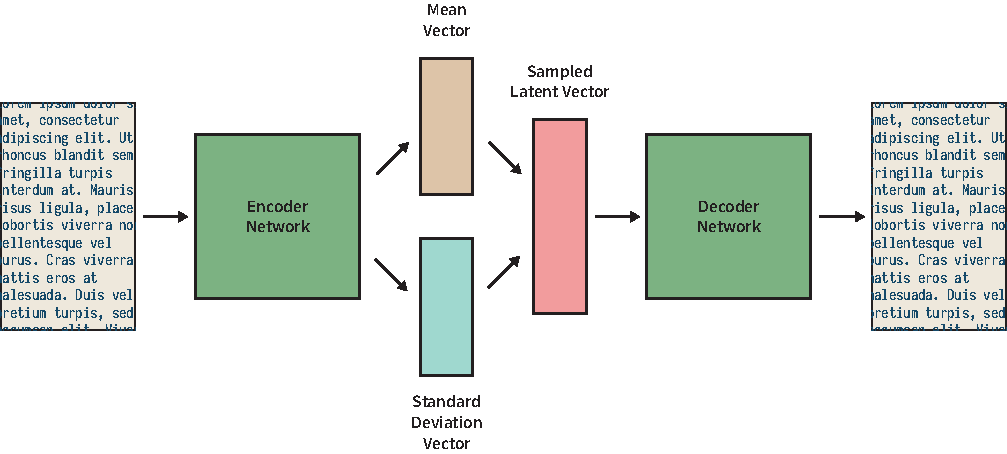
\includegraphics[width=150mm]{diagrams/variational_autoencoders.pdf}
	\caption{A simplified model diagram for a variational autoencoder, which takes as input some text, and it's predicted output being the same text as the input.\label{cum_growth}}
  \end{figure}

Due to the stochastic nature of the network, The loss function used for VAEs is specifically the Kullback–Leibler (KL) Divergence. KL measures the relative difference of two probability distributions.

$$
D_{KL}(P ||Q) = \sum_{x \subset X} P(x) \cdot log (\frac{P(x)}{Q(x)})
$$

In other words, it is the expectation of the logarithmic difference between the probabilities $P$ and $Q$, where the expectation of $P$ is understood.


\subsection{Conditional Variational Autoencoders}

Introduced by \cite{CVAEs are an improved model of the original VAE architecture by  conditioning on another description of the data, $y$. Samples can be generated from the conditional distribution $p(x|y)$. By changing the value of $y$, such as numbers of labels in MNIST, we can get corresponding samples $x \sim p(x|y)$.

However, it was found by \cite{du_variational_2018} that since the responses were generated from the same latent variable, it was not necessarily sufficent to model high-variability in responses. 

\subsection{Variational Autoregressive Decoders}

Introduced by \cite{du_variational_2018}, Variational Autoregressive Decoders (VADs) attempt to circumvent the sampling problem introduced from CVAEs by introducing latent variables in a autoregressive Decoder. At different time-steps, this allows the decoder to produce a multimodal distribution of text sequences, allowing a variety of responses to be produced.

% %%%%%%%%%%%%%%%%%%%%%%%%%%%%%%%%%%%%
% \chapter{Contribution}


% %%%%%%%%%%%%%%%%%%%%%%%%%%%%%%%%%%%%
% \chapter{Experimental Results}


% %%%%%%%%%%%%%%%%%%%%%%%%%%%%%%%%%%%%
% \chapter{Conclusion}


%% bibliography
\bibliographystyle{apa}
\bibliography{ref} 

\end{document}
